\subsubsection{UTXOs}
\label{subsec:utxos}
In the BSV blockchain, the Unspent Transaction Output (UTXO) model serves as the cornerstone for enabling transactions. Unlike traditional account-based models, where the state of an account is updated continuously, UTXOs are discrete data units that represent a specific amount of cryptocurrency \citep{antonopoulos2014mastering}. Each UTXO consists of its value in satoshis (the smallest unit of a Bitcoin) and a ScriptPubKey --- a cryptographic script that outlines the conditions for spending that particular UTXO. UTXOs are created as outputs from transactions and can be thought of as virtual "coins" that can be consumed or spent in subsequent transactions. When a UTXO is spent, it becomes an input for a new transaction, and the process creates new UTXOs as outputs, which in turn can be spent in the future.

The ScriptPubKey associated with each UTXO specifies the "locking script" that must be "unlocked" by a corresponding "unlocking script" or ScriptSig for the UTXO to be spent. Different types of ScriptPubKeys exist to facilitate various transaction types. Pay-to-Public-Key-Hash (P2PKH) \citep{p2pkh} is one of the most common types, designed for simple, one-to-one transactions. In a P2PKH output, the ScriptPubKey locks the UTXO with the hash of the recipient's public key. To spend it, the recipient must provide both the public key and a digital signature that proves ownership of the corresponding private key.

Pay-to-Script-Hash (P2SH) \citep{p2sh} offers more complexity and flexibility, enabling outputs to be locked with a hash of a script rather than a public key. P2SH allows for more complicated locking conditions, like multi-signature requirements or time-locked releases. In a P2SH transaction, the person who sets the conditions is not necessarily the one who fulfills them. This type enables functionalities like multi-signature wallets, where multiple parties must sign off on a transaction, or smart contracts that execute automatically under predetermined conditions.

Together, these UTXO features and ScriptPubKey types make up the rich ecosystem of transaction possibilities in the BSV blockchain, offering both robust security measures and versatile programmability.

\begin{figure}
    \centering
    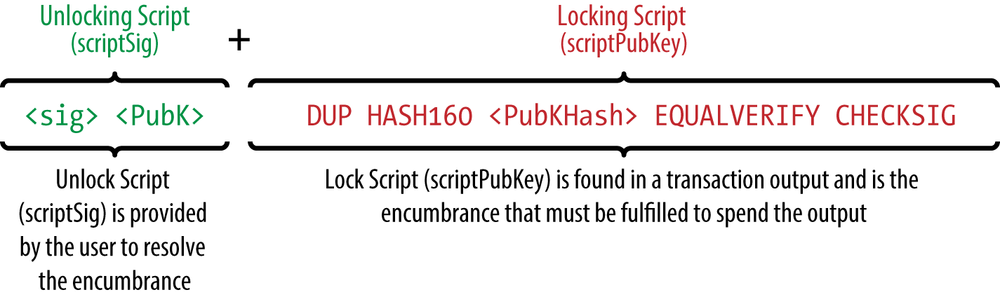
\includegraphics[width=\textwidth]{images/chapter-2/utxo.png}
    \caption[Unspent Transaction Output]{Reproduced from \citep{antonopoulos2014mastering}. Unspent Transaction Output, with a focus on the ScriptSig and ScriptPubKey components. ScriptSig serves as the 'unlocking script,' providing the necessary credentials to spend a UTXO. The ScriptPubKey acts as the 'locking script,' setting the conditions under which the UTXO can be spent. Together, these cryptographic scripts form the basis for secure and programmable transactions on the BSV blockchain.}
    \label{fig:utxo}
\end{figure}


